\documentclass[12pt,a4paper]{article}
\usepackage{verbatim}
\usepackage{graphicx}
\usepackage{float}
\author{ZHANG Xiao Research Intern in IBM CRL}
\title{Network 20q HW1}

\begin{document}
\maketitle
\pagebreak

\section{Distributed power control}

\subsection{a}
The basic formula of calculating SIR and P:
\begin{equation}
SIR_i[t] = \frac{G_{(i,i)}*P_i[t]}{\sum_{(j != i)} G_{(i,j)}*P_{j}[t] + noise}
\end{equation}
\begin{equation}
P_i[t+1] = \frac{\gamma_i}{SIR_i[t]} \times P_i[t]
\end{equation}
We could simplify them into matrix manipulation:
\begin{equation}
\vec{SIR[t]} = 1 \div ( (G \times \vec{P[t]} + noise) *  (1 \div (Diag(G) \cdot \vec{P[t]} )  )- 1 )
\end{equation}
\begin{equation}
\vec{P[t+1]} = \vec{\gamma} \div \vec{SIR[t]} * \vec{P[t]}
\end{equation}
In the formulas above, $\div$ means divide the value between two vectors in the same position, $*$ means multiply the value between two vectors in the same position, $\cdot$ means the dot production of two vectors.

And we could write the algrithm into matrix manipulation with the help of matlab or numpy.

The evolution of trasmit powers and received SIRs in ten timeslots are follows:

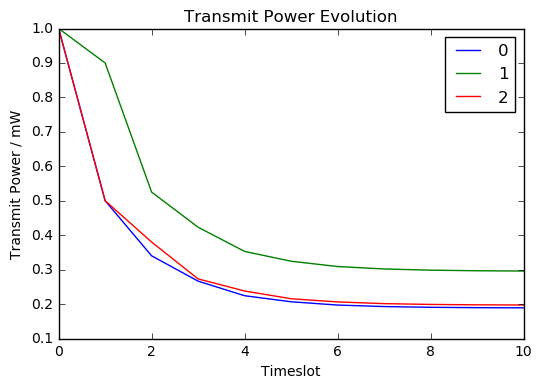
\includegraphics[width=\textwidth]{PIC/a-1.png}

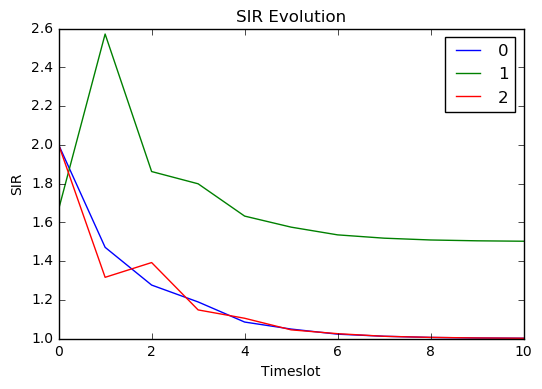
\includegraphics[width=\textwidth]{PIC/a-2.png}

In the end, hte power level would be [ 0.18900305,  0.2958567 ,  0.19723977],

SIR would be [ 1.00130033,  1.50202004,  1.00135969]

\subsection{b}

After last ten time slot, $\vec{p_0}$ would be [ 0.18900305,  0.2958567 ,  0.19723977,  1.        ],

The new evolution of trasmit powers and received SIRs in ten timeslots are follows:



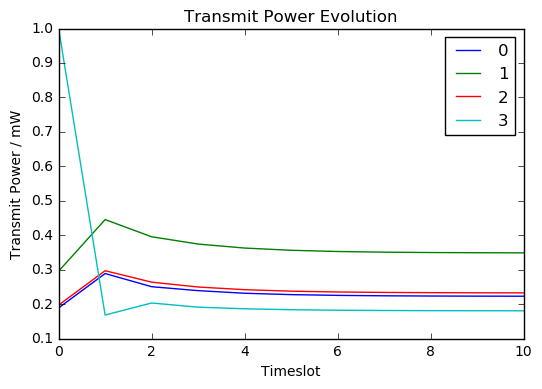
\includegraphics[width=\textwidth]{PIC/b-1.png}

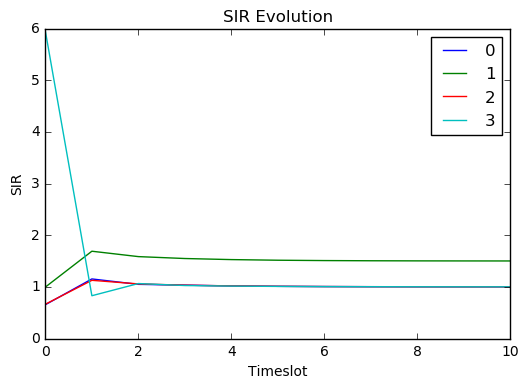
\includegraphics[width=\textwidth]{PIC/b-2.png}

At the end, the power level would be [ 0.22275949,  0.34867729,  0.23245153,  0.18046255],

SIR would be [ 1.00049425,  1.5007613 ,  1.00050754,  1.00040866].

Source code would be in another pdf file.

\end{document}